
\section{Conclusion}

\subsection{Lessons learned}

The experience of applying the data model language, the model
catalogue, and the associated generation tools in the context of
clinical research informatics has led to the following suggestions.

\textsl{A data dictionary is not enough}. A simple, flat list of data
definitions does not support re-use at scale: it requires the user to
place all of the contextual information into the definition of each
data item, and mitigates against the automatic generation and
application of definitions.  Instead, a compositional approach is
required, in which data elements are defined in explicit context.

\textsl{A catalogue is not enough}.  The models in the catalogue must
be linked to implementations, and to each other, with a considerable
degree of automatic support.  If the models are out of sync with the
implementations, and with the data, then their value is sharply
diminished.  If you are going to manage data at scale, you need a data
model-driven approach. 

\textsl{The tools must be usable by domain experts}. To have the
processes of model creation and maintenance mediated by software
engineers is problematic: there may be misunderstandings regarding
interpretation, but---more importantly---there are not enough software
engineers to go around.  The data models belong to the users. 

\textsl{There will be more models than you think}.  Different models
will be required for different types of implementation, and---in any
research domain, at least---data models will be constantly evolving,
with data being collected against different versions.  

\textsl{Intelligent, automatic support is essential}.  

\textsl{F} automate aspects of model management---versioning and dealing
  with multiple models
  \begin{itemize}
  \item automatically create (and propose) links, including
    classifications
  \item have links for new version of (sequential), refactoring of
    (parallel), derived from (data concepts across models), same as
    (strong assertion)
  \item use links in model maintenance - note that the definition that
    this was derived from has changed
  \item have publication cycle---a published model is for life
  \end{itemize}

\textsl{I} general lesson: if you have a model driven approach (data model
  or otherwise) then your management of models has all the same
  challenges as management of source code (you need an IDE) - really,
  if you are using models as programs, then you need to support them
  as programs

\clearpage

\begin{figure*}[h]
  \centering
  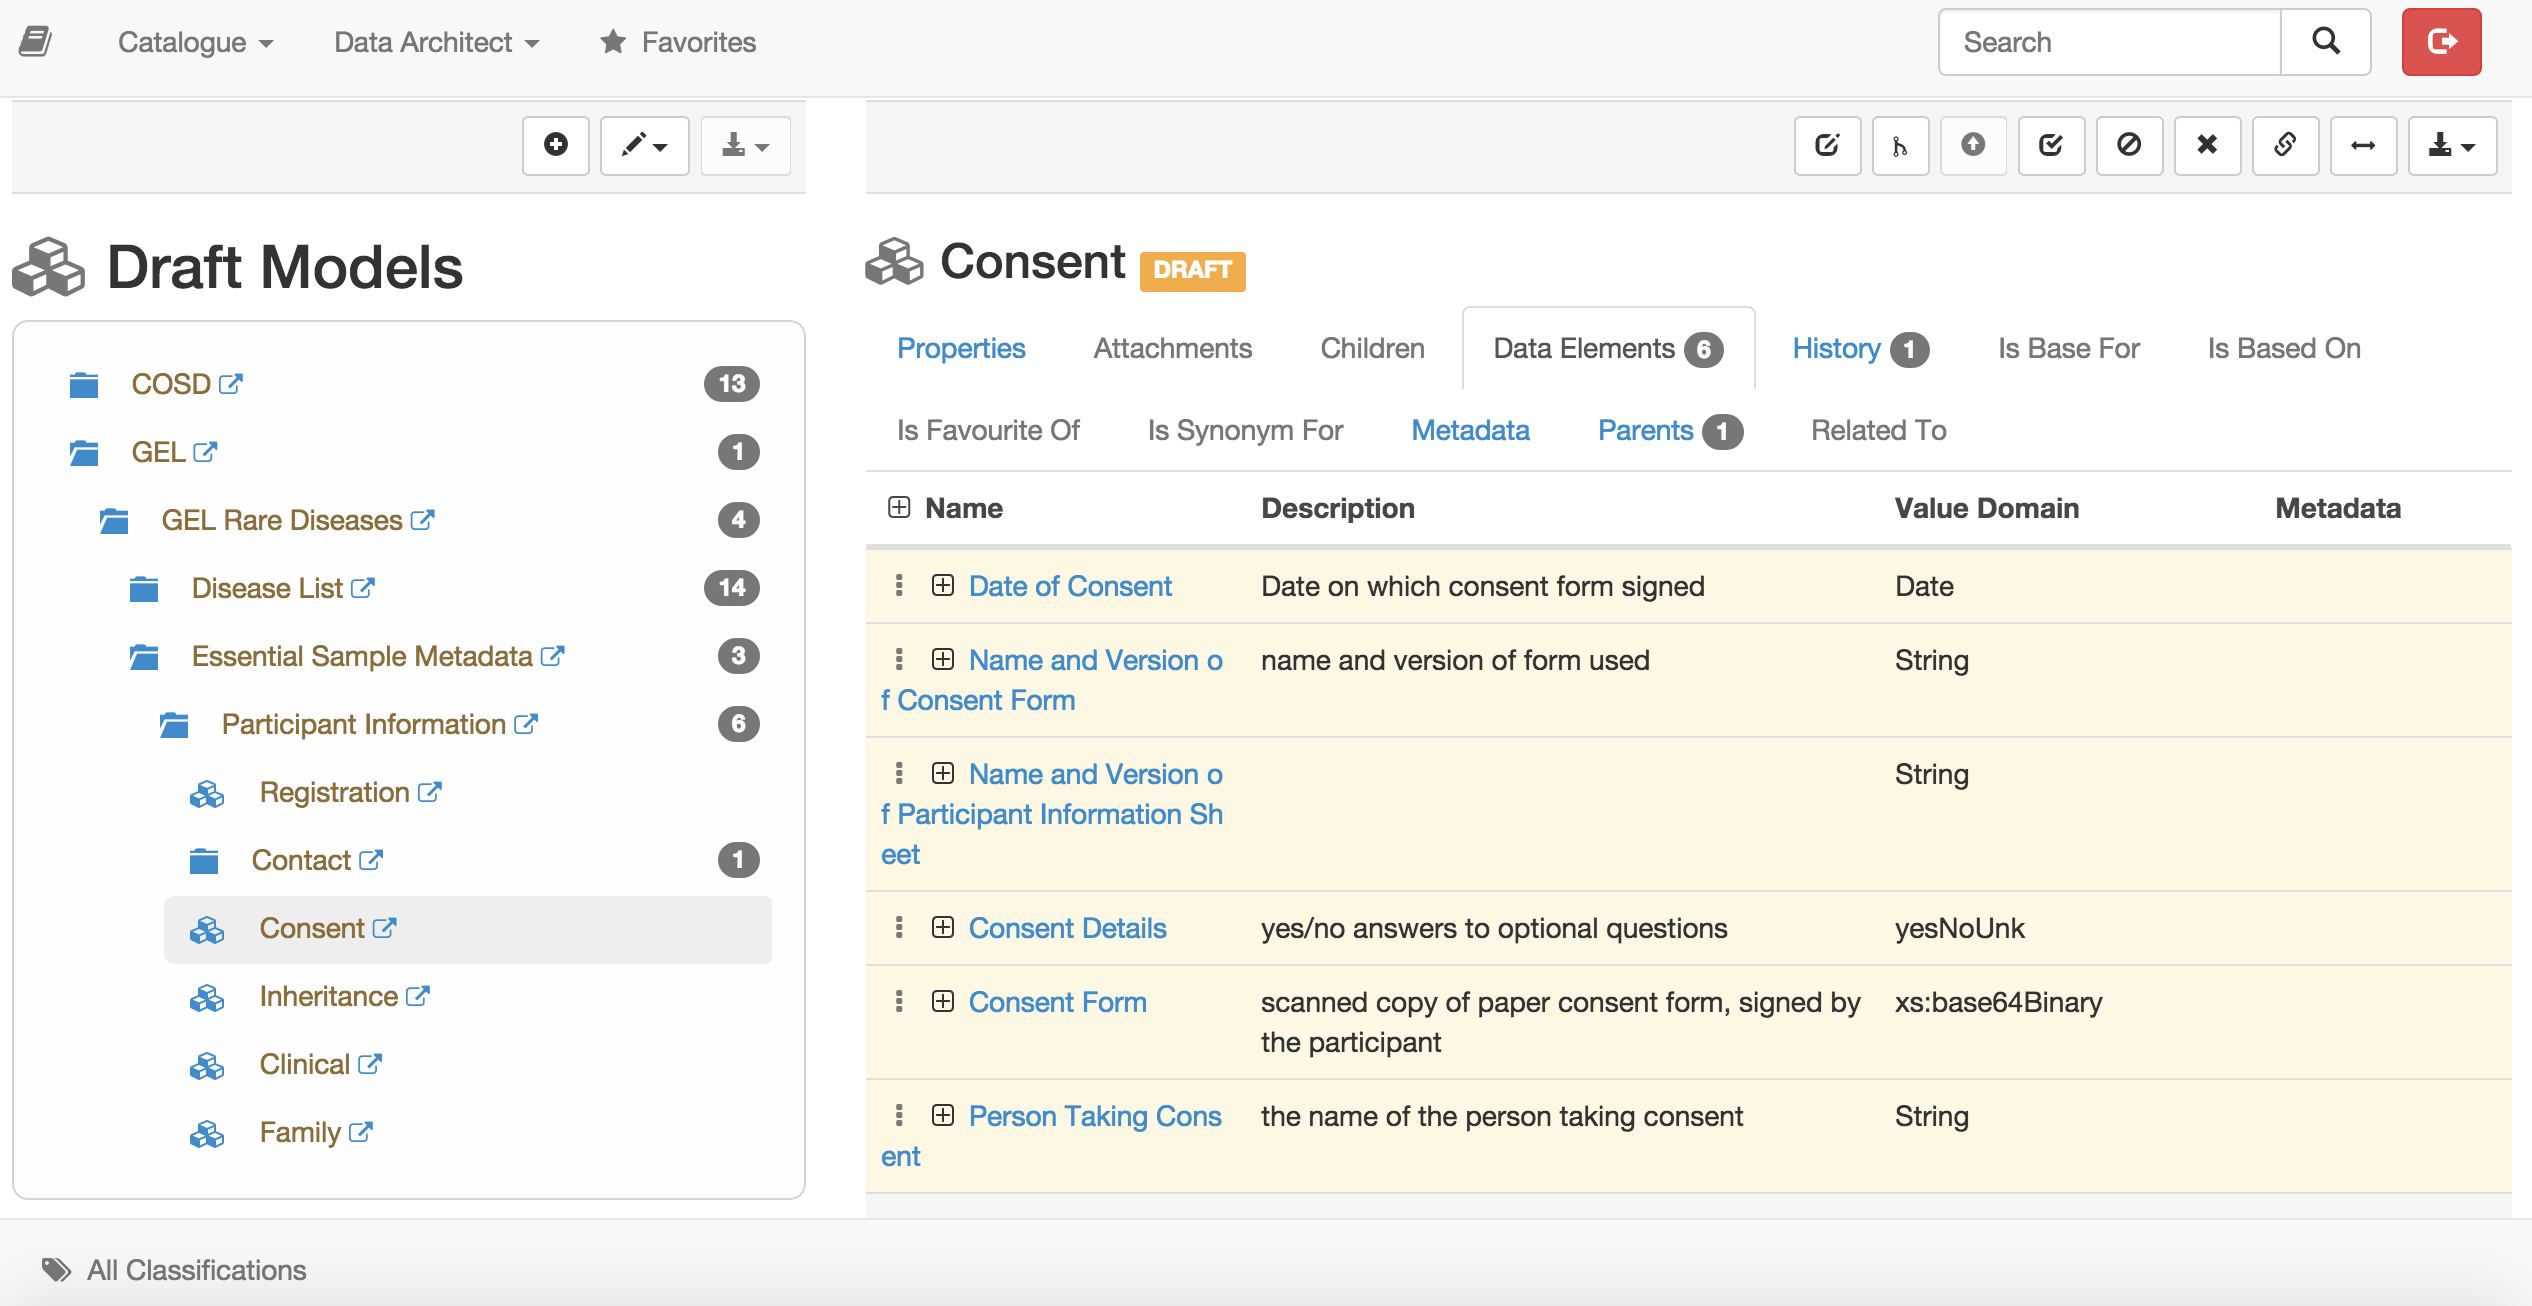
\includegraphics[width=\textwidth]{ScreenShot1}
  \caption{web interface to the model catalogue}
  \label{fig:webinterface}
\end{figure*}

\begin{figure*}[h]
  \centering
  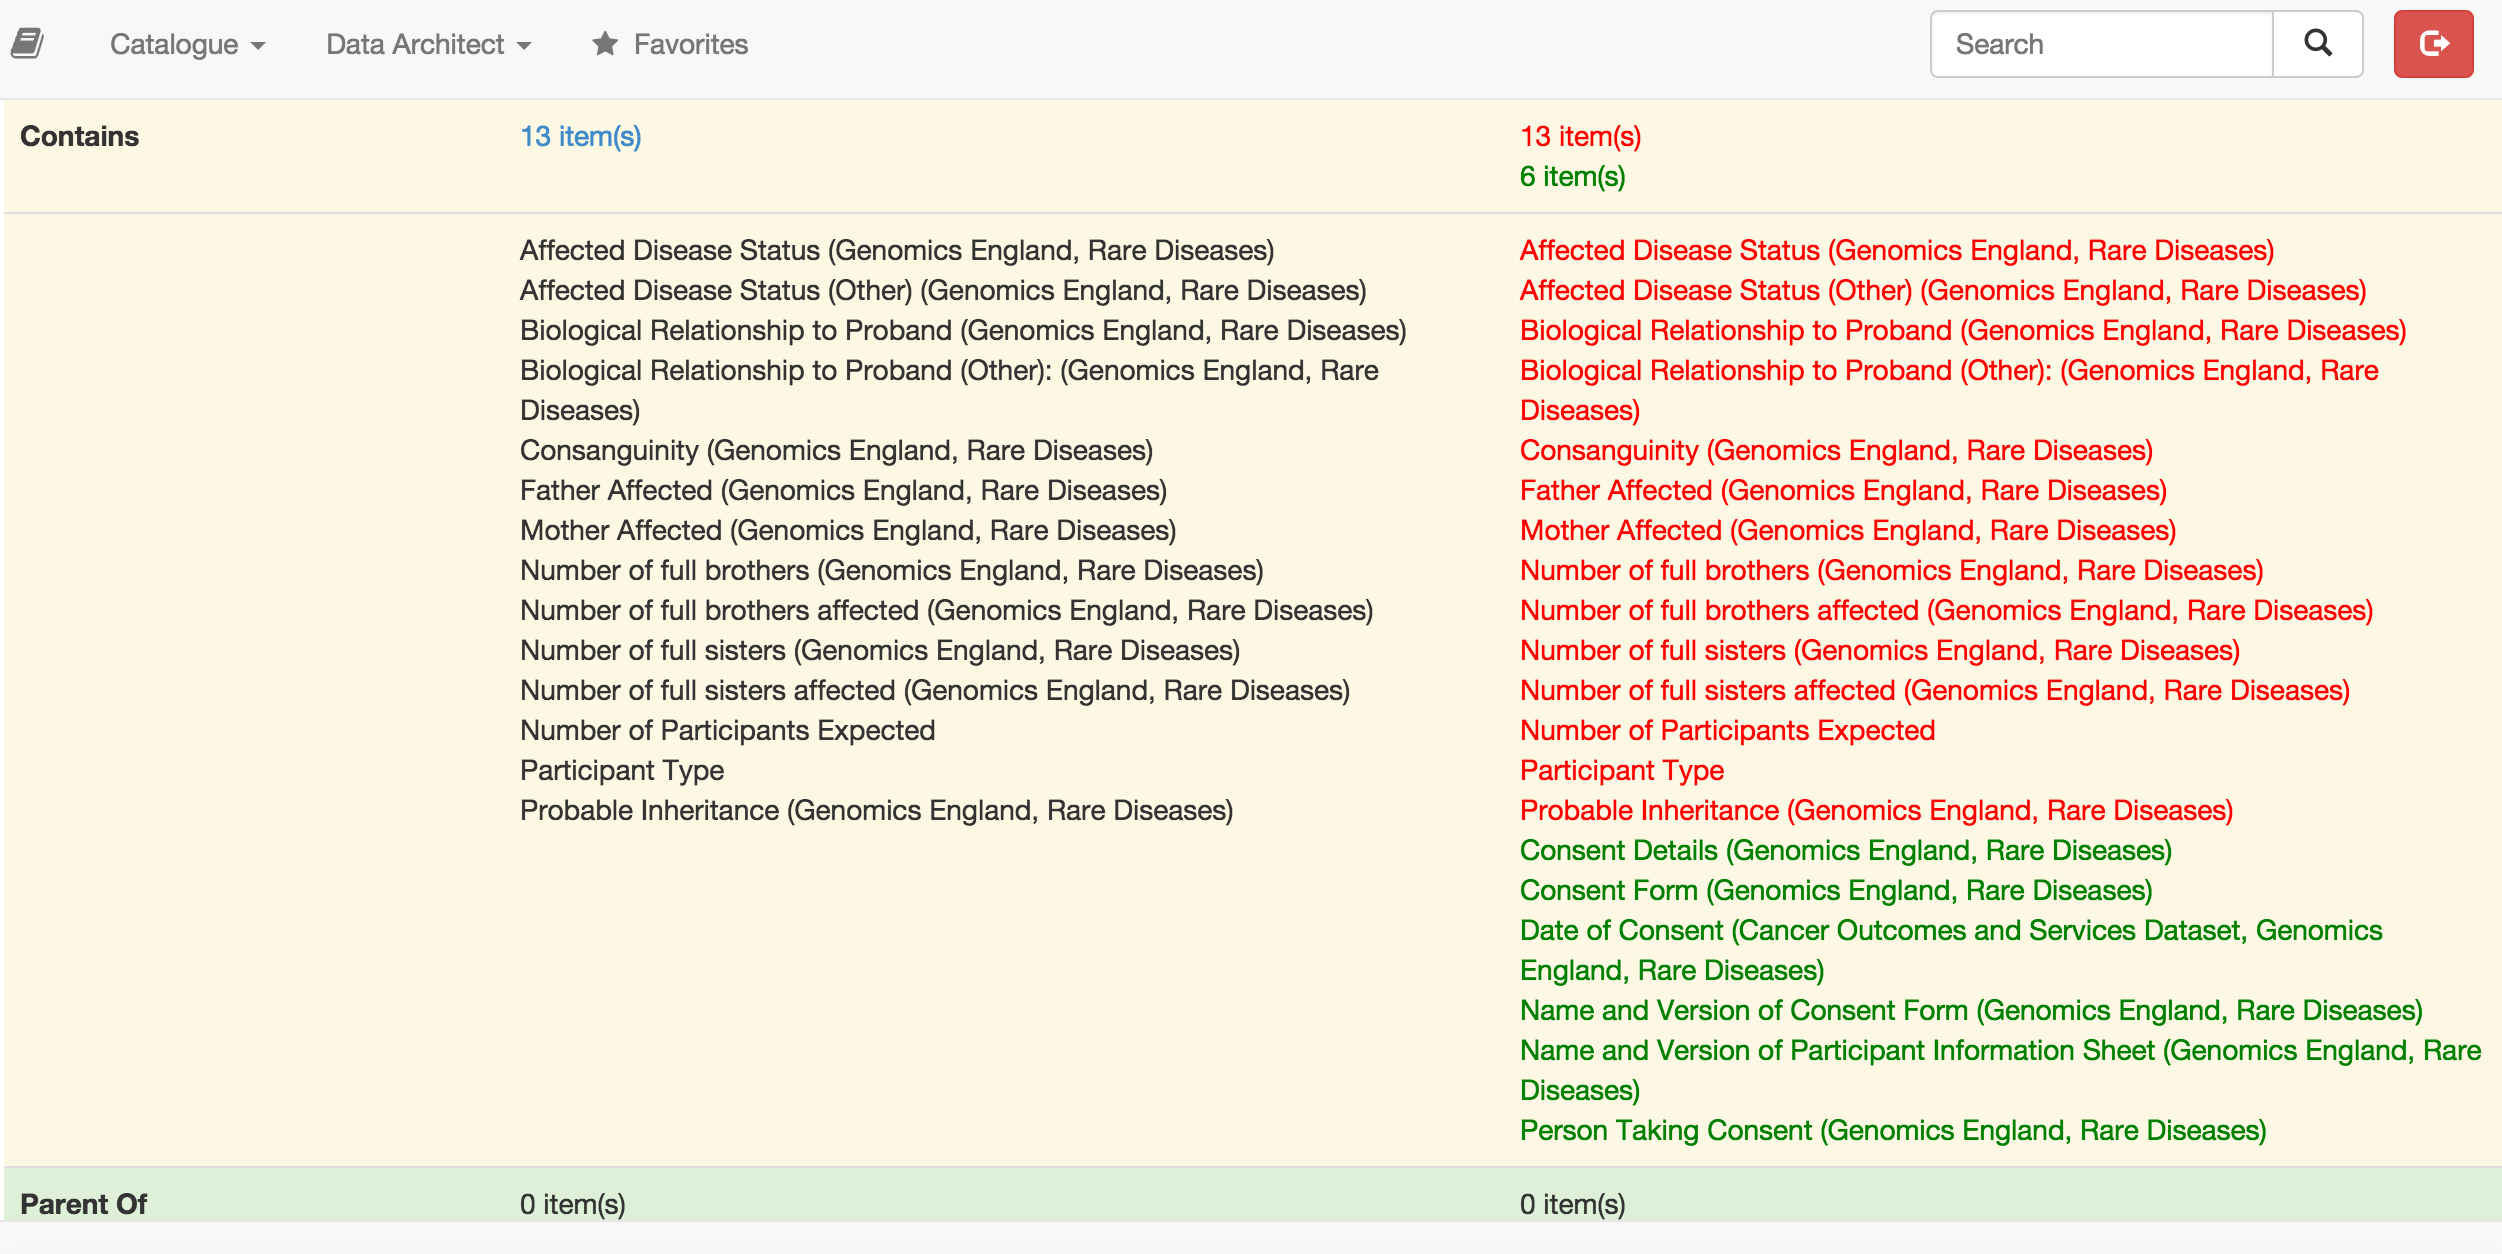
\includegraphics[width=\textwidth]{ScreenShot2}  
  \caption{automatic detection of model variation}
  \label{fig:variation}
\end{figure*}

